%\documentclass[honours,12pt,twoside]{unswthesis}

\usepackage{afterpage}
\usepackage{amsfonts}
\usepackage{amsmath}
\usepackage{amssymb}
\usepackage{amsthm}
\usepackage[english]{babel}
\usepackage{graphicx}
\usepackage{natbib}
\usepackage[utf8]{inputenc}
\usepackage{latexsym}
\usepackage{url}
\usepackage{todonotes}
\usepackage{tikz}
\usepackage{pdfpages}
\usetikzlibrary{arrows}
\usepackage{float}

\usepackage{booktabs}
\renewcommand{\arraystretch}{1.2}


%%%%%%%%%%%%%%%%%%%%%%%%%%%%%%%%%%%%%%%%%%%%%%%%%%%%%%%%%%%%%%%%%
%
%  The following are some simple LaTeX macros to give some
%  commonly used letters in funny fonts. You may need more or less of
%  these
%
\newcommand{\R}{\mathbb{R}}
\newcommand{\Q}{\mathbb{Q}}
\newcommand{\C}{\mathbb{C}}
\newcommand{\N}{\mathbb{N}}
\newcommand{\F}{\mathbb{F}}
\newcommand{\PP}{\mathbb{P}}
\newcommand{\T}{\mathbb{T}}
\newcommand{\Z}{\mathbb{Z}}
\newcommand{\B}{\mathfrak{B}}
\newcommand{\BB}{\mathcal{B}}
\newcommand{\M}{\mathfrak{M}}
\newcommand{\X}{\mathfrak{X}}
\newcommand{\Y}{\mathfrak{Y}}
\newcommand{\CC}{\mathcal{C}}
\newcommand{\E}{\mathbb{E}}
\newcommand{\cP}{\mathcal{P}}
\newcommand{\cS}{\mathcal{S}}
\newcommand{\A}{\mathcal{A}}
\newcommand{\ZZ}{\mathcal{Z}}

%%%%%%%%%%%%%%%%%%%%%%%%%%%%%%%%%%%%%%%%%%%%%%%%%%%%%%%%%%%%%%%%%%%%%
%
% The following are much more esoteric commands that I have left in
% so that this file still processes. Use or delete as you see fit
%
\newcommand{\bv}[1]{\mbox{BV($#1$)}}
\newcommand{\comb}[2]{\left(\!\!\!\begin{array}{c}#1\\#2\end{array}\!\!\!\right)
}
\newcommand{\Lat}{{\rm Lat}}
\newcommand{\var}{\mathop{\rm var}}
\newcommand{\Pt}{{\mathcal P}}
\def\tr(#1){{\rm trace}(#1)}
\def\Exp(#1){{\mathbb E}(#1)}
\def\Exps(#1){{\mathbb E}\sparen(#1)}
\newcommand{\floor}[1]{\left\lfloor #1 \right\rfloor}
\newcommand{\ceil}[1]{\left\lceil #1 \right\rceil}
\newcommand{\hatt}[1]{\widehat #1}
\newcommand{\modeq}[3]{#1 \equiv #2 \,(\text{mod}\, #3)}
\newcommand{\rmod}{\,\mathrm{mod}\,}
\newcommand{\p}{\hphantom{+}}
\newcommand{\vect}[1]{\mbox{\boldmath $ #1 $}}
\newcommand{\reff}[2]{\ref{#1}.\ref{#2}}
\newcommand{\psum}[2]{\sum_{#1}^{#2}\!\!\!'\,\,}
\newcommand{\bin}[2]{\left( \begin{array}{@{}c@{}}
				#1 \\ #2
			\end{array}\right)	}
%
%  Macros - some of these are in plain TeX (gasp!)
%
\newcommand{\be}{($\beta$)}
\newcommand{\eqp}{\mathrel{{=}_p}}
\newcommand{\ltp}{\mathrel{{\prec}_p}}
\newcommand{\lep}{\mathrel{{\preceq}_p}}
\def\brack#1{\left \{ #1 \right \}}
\def\bul{$\bullet$\ }
\def\cl{{\rm cl}}
\let\del=\partial
\def\enditem{\par\smallskip\noindent}
\def\implies{\Rightarrow}
\def\inpr#1,#2{\t \hbox{\langle #1 , #2 \rangle} \t}
\def\ip<#1,#2>{\langle #1,#2 \rangle}
\def\lp{\ell^p}
\def\maxb#1{\max \brack{#1}}
\def\minb#1{\min \brack{#1}}
\def\mod#1{\left \vert #1 \right \vert}
\def\norm#1{\left \Vert #1 \right \Vert}
\def\paren(#1){\left( #1 \right)}
\def\qed{\hfill \hbox{$\Box$} \smallskip}
\def\sbrack#1{\Bigl \{ #1 \Bigr \} }
\def\ssbrack#1{ \{ #1 \} }
\def\smod#1{\Bigl \vert #1 \Bigr \vert}
\def\smmod#1{\bigl \vert #1 \bigr \vert}
\def\ssmod#1{\vert #1 \vert}
\def\sspmod#1{\vert\, #1 \, \vert}
\def\snorm#1{\Bigl \Vert #1 \Bigr \Vert}
\def\ssnorm#1{\Vert #1 \Vert}
\def\sparen(#1){\Bigl ( #1 \Bigr )}

\newcommand\blankpage{%
    \null
    \thispagestyle{empty}%
    \addtocounter{page}{-1}%
    \newpage}
    
%%%%%%%%%%%%%%%%%%%%%%%%%%%%%%%%%%%%%%%%%%%%%%%%%%%%%%%%%%%%%%
%
% These environments allow you to get nice numbered headings
%  for your Theorems, Definitions etc.  
%
%  Environments
%
%%%%%%%%%%%%%%%%%%%%%%%%%%%%%%%

\newtheorem{theorem}{Theorem}[section]
\newtheorem{lemma}[theorem]{Lemma}
\newtheorem{proposition}[theorem]{Proposition}
\newtheorem{corollary}[theorem]{Corollary}
\newtheorem{conjecture}[theorem]{Conjecture}
\newtheorem{definition}[theorem]{Definition}
\newtheorem{example}{Example}
\newtheorem{remark}[theorem]{Remark}
\newtheorem{question}[theorem]{Question}
\newtheorem{notation}[theorem]{Notation}
\numberwithin{equation}{section}

%\begin{document}

\chapter{Results}\label{results}

\section{Final model structure}

The final simplified model has a similar structure to that of Ghafoorian et al.'s candidate detection model \cite{GhafoorianM.2017Dml3}. The model structure is shown in Figure \ref{results-model-fig}. The input data contains two axial images: soft tissue extracted T1 and \textsc{flair} images. Each of the images has resolution 51$\times$51 pixels and is centred at the same coordinate. The model classifies the central pixel as either a positive or negative reading, formatted as a two-dimensional vector. A response of $(1,0)^\intercal$ indicates a positive (lacune) sample and $(0,1)^\intercal$ a negative (non-lacune) sample.

% Simplified model structure
\begin{figure}[ht]
	\centering
	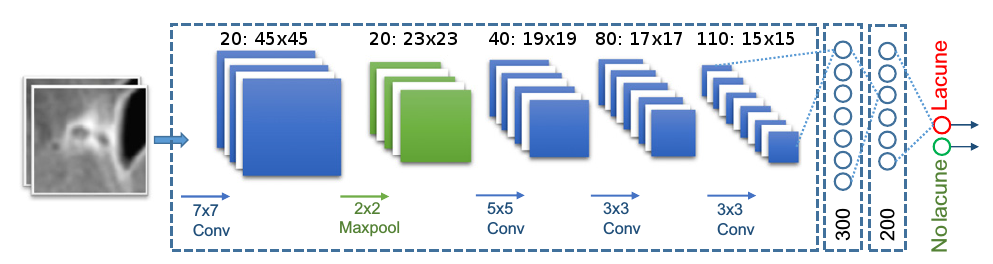
\includegraphics[width=\linewidth]{Images/7_simplified_model.png}
	\caption{Simplified model structure.}
	\small Image adapted from \cite{GhafoorianM.2017Dml3}
	\label{results-model-fig}
\end{figure}

The model consists of four convolutional layers of size 20, 40, 80 and 110, with filter sizes 7$\times$7, 5$\times$5, 3$\times$3 and 3$\times$3 respectively. A single max pooling layer is placed after the first convolutional layer, with size 2$\times$2 and stride 2. The convolutional layers are followed by three fully connected layers of size 300, 200 and 2. The final layer has softmax activation to output a probability distribution. All other layers have ReLU activation in order to avoid the vanishing gradient problem (see Section \ref{nnet-vanishinggradprob}). All neurons undergo batch normalisation and are initialised using the He method \cite{HeKaiming2015DDiR}. A dropout rate of 0.3 was applied to the fully connected layers.

Training was conducted using stochastic gradient descent with the Adam optimiser and a batch size of 128. A decaying learning rate was set from $5\times10^{-4}$ to $1\times10^{-6}$ by the 40th epoch. Cross-entropy loss was used with L2-regularisation, with the penalty rate set to $1\times10^{-4}$. An early stopping mechanism was implemented such that the model is tested against the validation set at the end of each epoch. If the validation accuracy improves, the model is saved. Once 40 epochs have run, the final saved model will have the highest validation accuracy.

Two models were trained using different positive-negative response ratios. The first model was developed using the positive-negative response ratio described by Ghafoorian et. al \cite{GhafoorianM.2017Dml3}: one third positive and two thirds negative. There are only 3846 positive samples in the MAS data set, allowing for a random selection of 7692 negative samples, thus giving a total sample size of 11538. These samples were split into three data sets: training, validation and testing. Splitting the data into these groups at a ratio of 50:25:25 yielded sample sizes 5769, 2884 and 2885 respectively.

The second model used the entire developed set of positive and negative lacune samples. This consisted of 3846 positive and 39983 negative samples to give a total sample size of 43829. Positive samples encompass 8.78\% of data samples. Similarly to the first data set, the data was split into training, validation and testing sets using a ratio of 50:25:25. This yielded sample sizes 21914, 10957 and 10958 respectively. All data sets were saved as R data files (\texttt{.Rda}).


\section{Training environment}

Model code was developed in R (v3.5.0) using RStudio (v1.1.453). The neural network was built and trained using Tensorflow (v1.10.0) through the R interface \texttt{tensorflow} (v1.8). The model was trained on a Linux machine running Ubuntu (release 16.04). The Tensorflow model was trained on the machine's CPU, an Intel(R) Core(TM) i7-4790 CPU 3.60GHz, with 16GB of RAM. 

\section{Results}

\subsection*{First model}

The first model generated has the same positive-negative sample ratio as outlined by Ghafoorian et. al \cite{GhafoorianM.2017Dml3}. The data consists of one-third positives and two-thirds negatives.

The model was trained for 40 epochs over 24 minutes, adjusting the network weights with each batch of 128 samples. Reusing the same data samples a large number of times introduces overfitting into the network \cite{Goodfellow-et-al-2016}. Overfitting can be observed when the accuracy of the training data set becomes very high, whereas the accuracy of the validation and testing data sets are low. Hence assessing model training accuracy can efficiently convey early model improvement; however it is not indicative of the model's performance when given new data.

Training accuracy was calculated every 5 batches, where each batch contained 128 samples. The resulting accuracies are shown in Figure \ref{results-train-acc4-fig}. There is a rapid increase in training accuracy within the first 100 batches. The model improvement occurs in steps as new features are found and more precise weight changes are made with the lowering learning rate \cite{Folly2009, Nielson2015}. The model reports a 100\% training accuracy consistently by batch 300. A majority of the model training occurs very early. In later training epochs, the training cost and learning rates are low and so the change in weights is also low (see Section \ref{nnets-backprop} on Backpropagation).

% Training accuracy
\begin{figure}[hb]
	\centering
	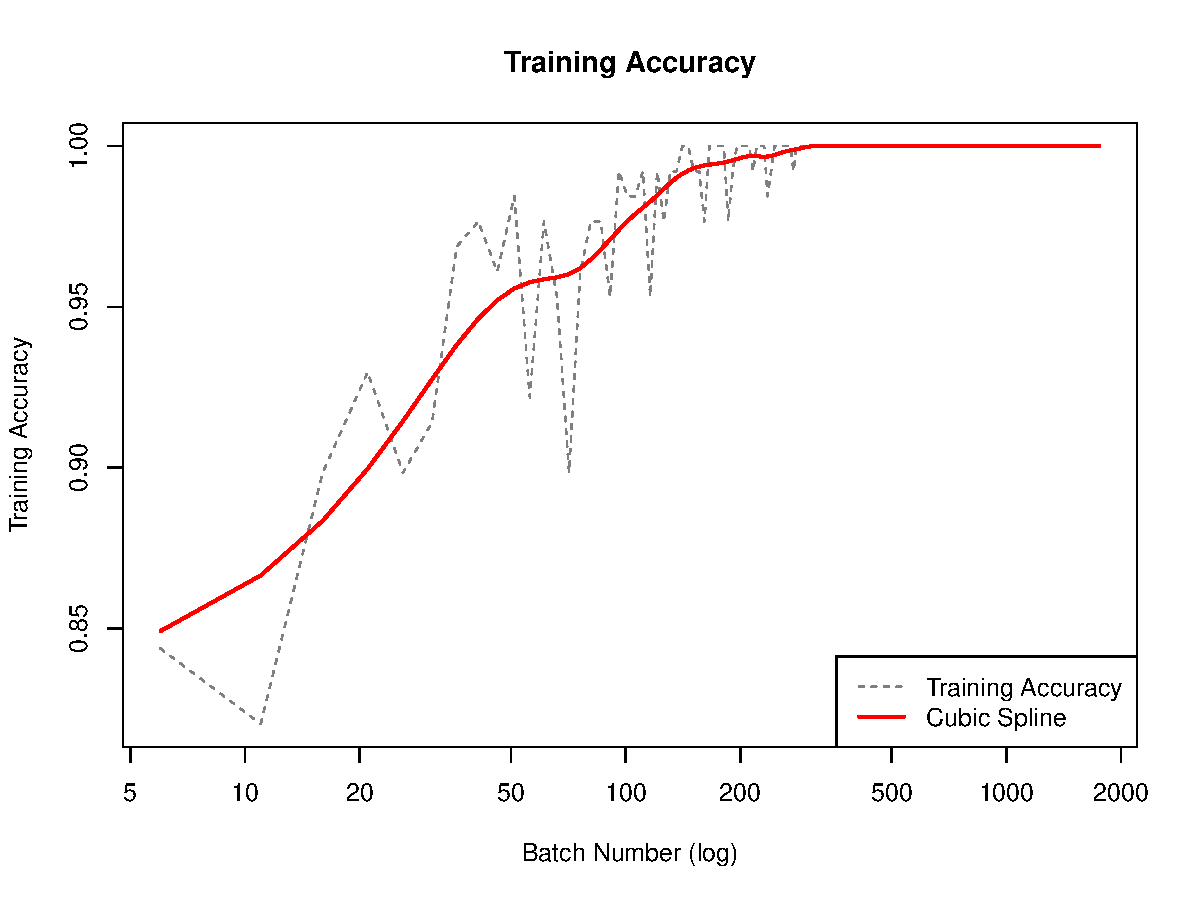
\includegraphics[width=\textwidth]{Images/7_train_acc4.pdf}
	\caption{Training data accuracy logged every 5 batches.}
	\label{results-train-acc4-fig}
\end{figure}

The model's validation set accuracy was tested after each epoch. This data set was not used for training and is used to assess the model's performance given new unseen data. The resulting validation accuracies are shown in Figure \ref{results-valid-acc4-fig}. Validation accuracy increases rapidly within the first 10 epochs. The maximum validation accuracy occurred at epochs 18, 22 and 25, achieving an accuracy of 0.992. The model was saved at epoch 18 to help minimise overfitting that may occur at later epochs. Applying this best validation accuracy model to the test data set resulted in an accuracy of 0.994.

% Validation accuracy
\begin{figure}[hb]
	\centering
	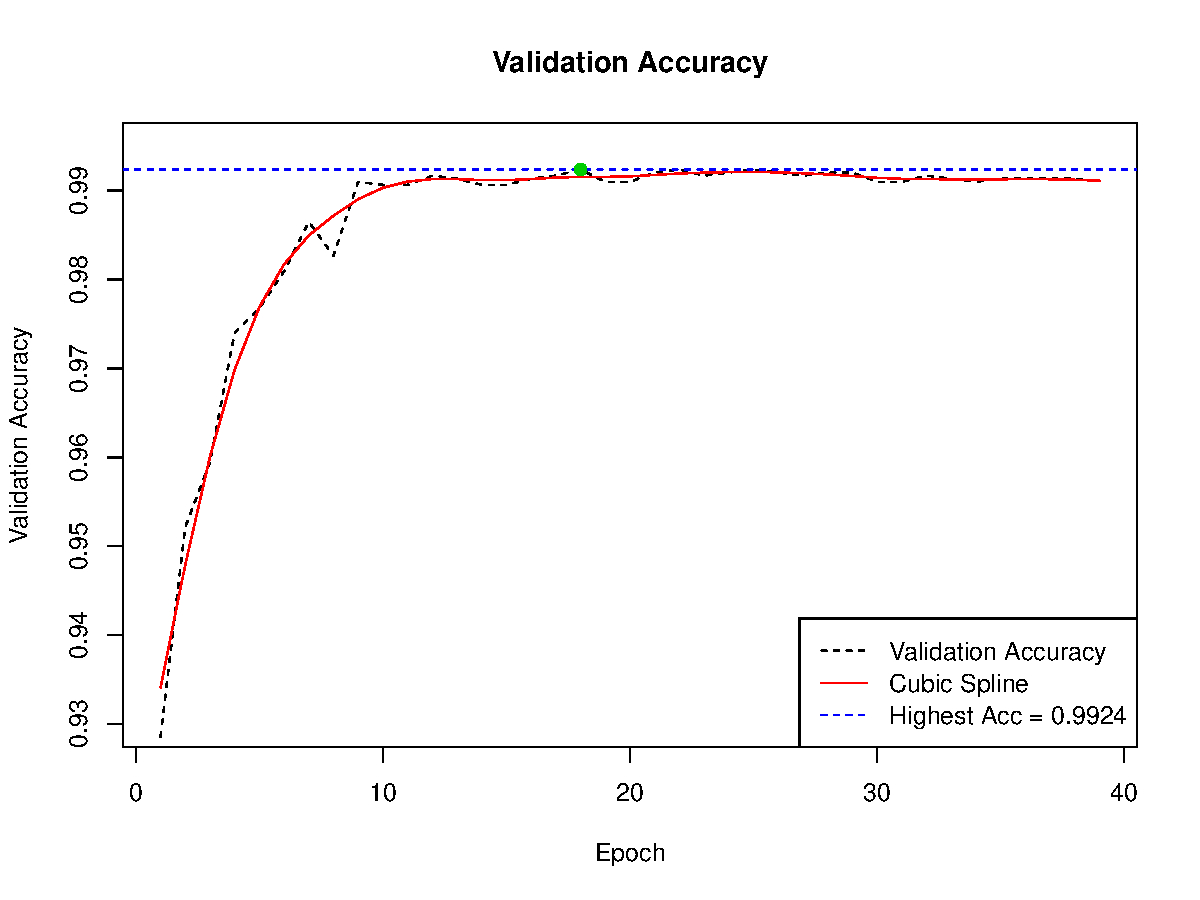
\includegraphics[width=\textwidth]{Images/7_valid_acc4.pdf}
	\caption{Validation data accuracy logged after each epoch.}
	\label{results-valid-acc4-fig}
\end{figure}

Though overall accuracy is a strong indicator of model performance, some types of inaccuracy can be more detrimental than others. In the identification of lacunes, it is preferable to have a larger number of false candidate lacunes than misclassify a true lacune. As a result, models will be compared by considering actual and predicted classification differences. Using this scheme, there are four outcomes: true-positive, true-negative, false-positive, and false-negative. These outcomes can be formatted into a \textit{confusion matrix}, as shown in Table \ref{results-confmat4-tab}.

\begin{table}[ht]
	\centering
	\begin{tabular}{@{}lll@{}}
	\toprule[1.5pt]
	& Positive & Negative\\
	\midrule
	True & 1004 & 1863\\
	False & 16 & 2\\
	\bottomrule[1.5pt]\\
	\end{tabular}
	\caption{Confusion matrix of the Model 1 testing data set.}
	\label{results-confmat4-tab}
\end{table}

The sensitivity of the model to lacunes is 99.6\% and specificity (correct classification of negative samples) of non-lacunes is 98.4\%.

\subsection*{Second model}

The second model was built using all of the generated positive and negative samples as described in Section \ref{data-samples}. The resulting training accuracy is shown in Figure \ref{results-train-acc5-fig}. The additional noise present in comparison to the previous model is the result of the larger sample size, rising from 5769 to 21914 samples. Note that the batch size and number of training epochs remained at 128 and 40 respectively, resulting in a larger number of batches processed during training. Model training duration was 85 minutes. The behaviour of this model was similar to that of the previous model, with a steep increase in training accuracy in early epochs followed by consistent correct classifications. Training accuracy was consistently at 100\% by batch 1000. 

% Training accuracy
\begin{figure}[ht]
	\centering
	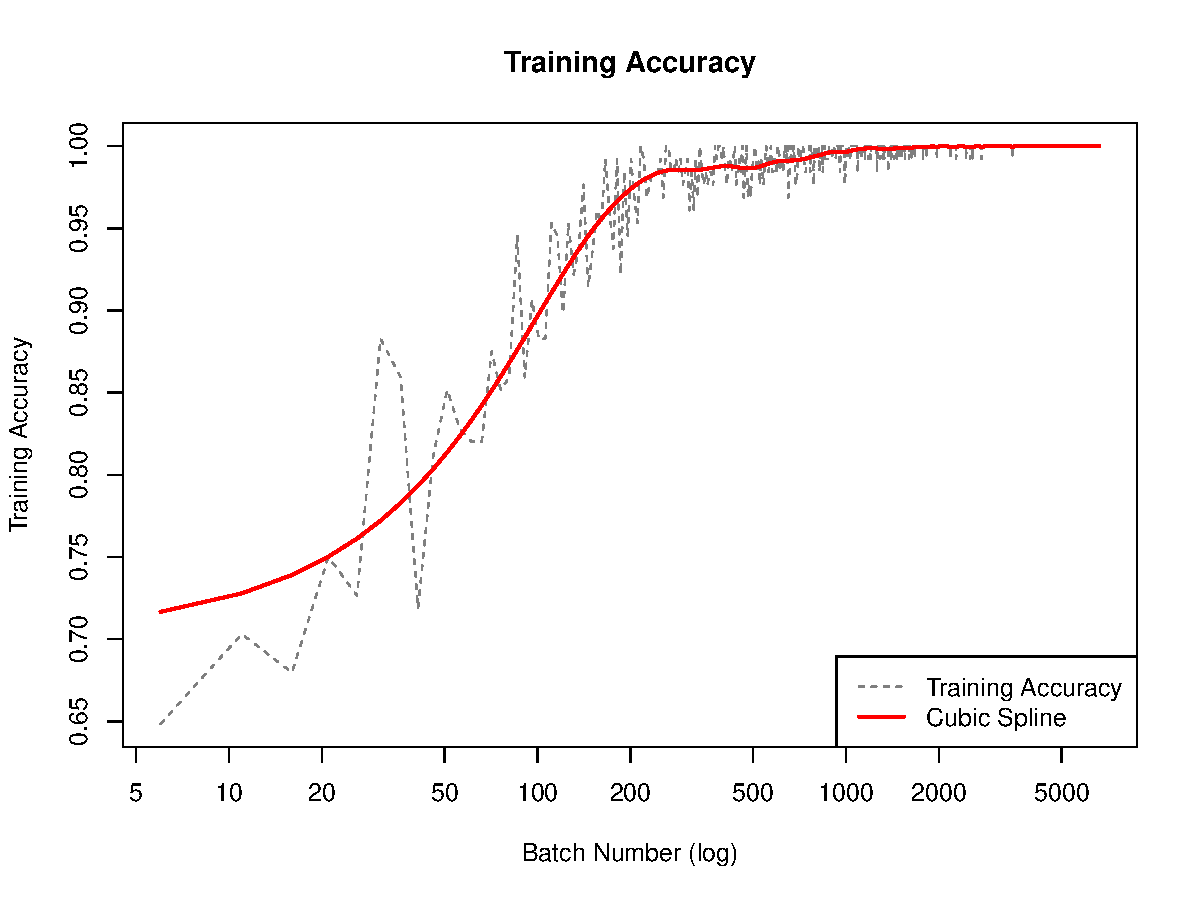
\includegraphics[width=\textwidth]{Images/7_train_acc5.pdf}
	\caption{Training data accuracy logged every 5 batches.}
	\label{results-train-acc5-fig}
\end{figure}

The performance of the model on the validation set is given in Figure \ref{results-valid-acc5-fig}. Validation accuracy was maximised at epochs 28 and 34, achieving an accuracy of 0.998. The model was saved at the earlier epoch 28 to reduce overfitting.

% Validation accuracy
\begin{figure}[ht]
	\centering
	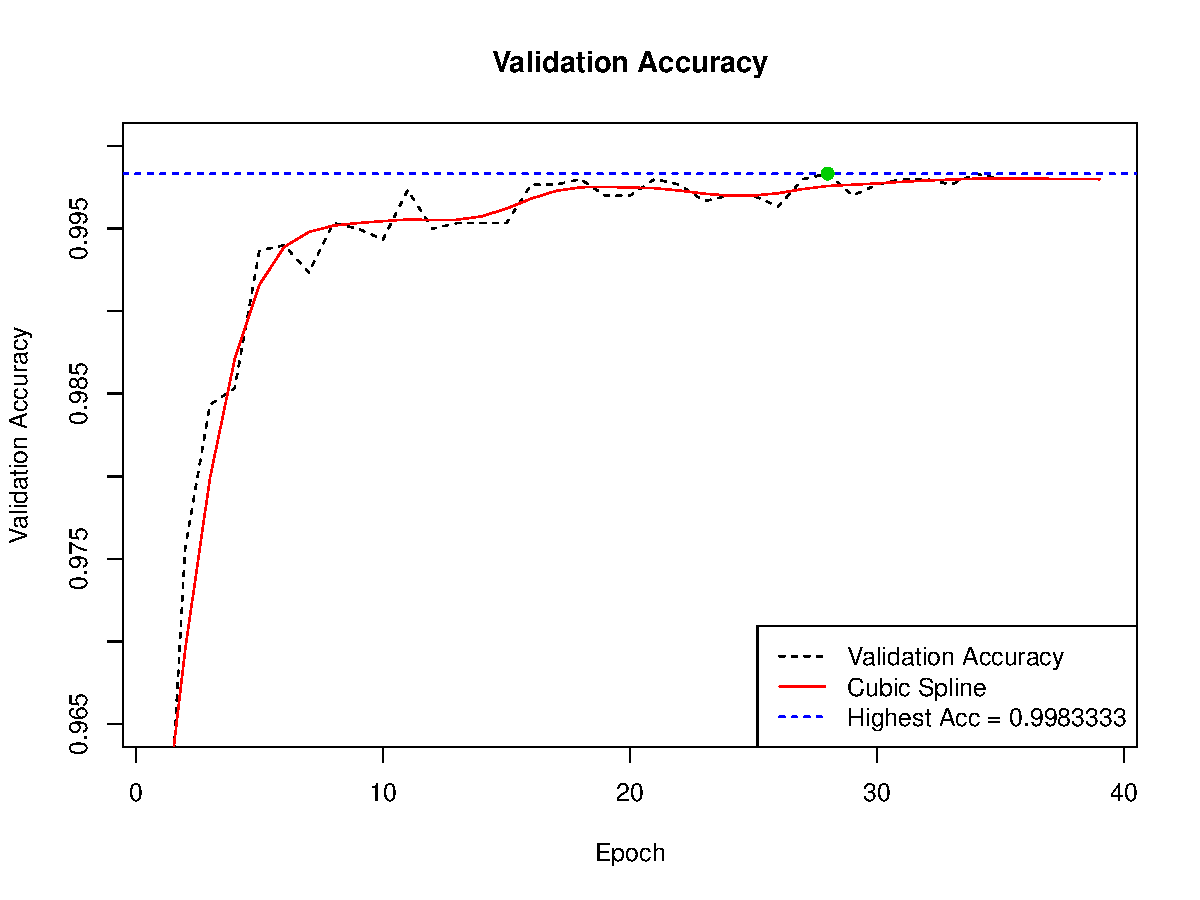
\includegraphics[width=\textwidth]{Images/7_valid_acc5.pdf}
	\caption{Validation data accuracy logged after each epoch}
	\label{results-valid-acc5-fig}
\end{figure}

Applying this best validation accuracy model to the test set achieved an accuracy of 99.8\%. The confusion matrix is given by Table \ref{results-confmat5-tab}, to give a sensitivity of 99.9\% and specificity of 99.7\%.

\begin{table}[ht]
	\centering
	\begin{tabular}{@{}lll@{}}
	\toprule[1.5pt]
	& Positive & Negative\\
	\midrule
	True & 961 & 9977\\
	False & 19 & 1\\
	\bottomrule[1.5pt]\\
	\end{tabular}
	\caption{Confusion matrix of the Model 2 testing data set.}
	\label{results-confmat5-tab}
\end{table}

\subsection*{Model comparisons}

The sensitivities and specificities of the two models are given in Table \ref{results-sens-spec-tab}. We observe that the second trained model has a higher sensitivity and specificity than that of the first model. We conduct a hypothesis test on the differences between the two models.

\begin{table}[ht]
	\centering
	\begin{tabular}{@{}lll@{}}
	\toprule[1.5pt]
	& Sensitivity & Specificity\\
	\midrule
	Model 1 & 0.9980 (1004/1006) & 0.9915 (1863/1879)\\
	Model 2 & 0.9990 (961/962) & 0.9981 (9977/9996)\\
	\bottomrule[1.5pt]\\
	\end{tabular}
	\caption{Sensitivities and specificities of both models.}
	\label{results-sens-spec-tab}
\end{table}

First, we test the difference in sensitivity proportions. The Central Limit Theorem (\textsc{clt}) is not applicable as the number of false-negatives is too small in both models. Instead, we use Fisher's Exact test. Let $X_1$ and $X_2$ be the number of lacunes correctly identified under the first and second models respectively. Let $n_1$ and $n_2$ be their respective sample sizes. Under the null hypothesis, for fixed $X_1 + X_2$, $X_1$ and $X_2$ have a hypergeometric distribution with probability
\begin{align*}
	P(X_1 = x_1, X_2 = x_2) = \dfrac{\dbinom{n_1}{x_1}\dbinom{n_2}{x_2}}{\dbinom{n_1 + n_2}{x_1 + x_2}}.
\end{align*}

The resulting p-value is 1, and we conclude that the two sensitivity proportions are not significantly different.

We now test the difference in specificity rates. We hypothesise that both sample proportions come from sampling distributions with the same probability. We can apply a $z$-test since we have sufficiently large number of observations and the data are independent. Let $X_1$ and $X_2$ be the number of correctly classified negative samples from the first and second models respectively. Let $n_1$ and $n_2$ be the total number of negative samples, so that $\hat{p}_1 = \dfrac{X_1}{n_1}$ and $\hat{p}_2 = \dfrac{X_2}{n_2}$ are the observed specificities. The observed pooled specificity proportion is
\begin{align*}
	\hat p_{pooled} = \dfrac{1863+9977}{1879+9996} = 0.9970526.
\end{align*}
From the \textsc{clt},
\begin{align*}
	Z = \dfrac{\hat{p}_1 - \hat{p}_2}{\sqrt{p_{pooled}(1 - p_{pooled})\left(\frac{1}{n_1} + \frac{1}{n_2}\right)}} \approx \mathcal{N}(0,1).
\end{align*}
The resulting test statistic is $z = -4.852599$. The probability of the observed proportion difference or lower is given by $P(Z < z) = 6.09\times10^{-7}$. This is well below the 5\% significance level and it is concluded that the specificity of the second model is higher than that of the first.

It has been proven that the model trained with the larger sample size and smaller proportion of positives did not affect sensitivity rates and increased specificity. 

\todo[inline]{Show examples of false-positives and true-negatives. What do these tend to look like?}

\todo[inline]{What happens when the scan is run on a whole brain?}

%\section{Reference Model Results}
%
%Results from running Ghafoorian's model. Training time, and final sensitivity and average false-positives per slice.
%
%\subsection*{Attempt1}
%
%training/testing in ratio 70:30. Here, only 7\% of data consists of positives. 41819 samples in total. Validation occurs on first 500 of the testing set. Training time: 02:04:48.
%Training accuracy achieved 100\% before batch 100x5. Validation accuracy peaked at epoch 8, with an accuracy of 100\%. Though should be noted that the size of this validation set consists of only 500 samples. Testing the whole testing set (15544 samples) achieves an accuracy of 0.9938.
%
%\subsection*{Attempt2}
%
%training/validation/testing in ratio 50:25:25. 1/3 of data was positives. 11539 samples in total. Training time: 00:23:11.
%Training accuracy achieved 100\% before batch 50x5. Validation accuracy peaked at epoch 21, which achieved an accuracy of 0.984055. Applying this best validation model to testing data achieved an accuracy of 0.9833622. Lower accuracy could be the result of fewer data points for training - caused by having only a limited number of positives in the original data set compared to the abundant negatives.
%
%\subsection*{Attempt3}
%
%Use original 7\% ratio. 41819 samples, with training/validation/testing in ratio 50:25:25. Have to be careful not to introduce too many negatives as this could impact what the model attempts to predict. E.g. if there are only 1\% positives, then an accuracy of 99\% could be achieved just by labelling all the samples as negative. Training time: 01:58:23.
%Training accuracy achieved 100\% before batch 100x5. Validation accuracy peaked at epoch 18, with an accuracy of 0.9979159, with the set containing 12955 samples. The testing set achieved an accuracy of 0.9972.
%
%\subsection*{Fixed Samples}
%
%Samples were changed. Previously, negative samples were chosen such that they were not lacunes, and also did not have a central pixel value of 0. However, some regions within the brain matter do have a central value of 0, and these can be some of the hardest points to distinguish.
%
%Negative sampling was changed to random points that were not lacunes, and the entire 9x9 central square is not 0 (to remove samples from outside the brain matter). 
%
%\subsection*{Attempt4}
%
%training/validation/testing in ratio 50:25:25. 1/3 of data was positives. 11538 samples in total. Training time: 00:22:51.
%Training accuracy achieved 100\% at batch 28x5. Consistent 100\% by batch 50x5. Validation accuracy peaked at epochs 31 and 34, achieving an accuracy of 0.9899445. Applying this best validation accuracy model to the test set achieved an accuracy of 0.9885615.
%
%Testing set was only 2885 samples. The number of true/false-positives and negatives were:
%TP: 972
%TN: 1879
%FP: 30
%FN: 4
%
%Sensitivity is 972/(972+4) = 99.6\% and specificity is 1879/(1879+30) = 98.4\%.
%
%
%
%\subsection*{Attempt5}
%
%training/validation/testing with 8.77\% positives. 43854 samples in total. Training time: 01:13:17. Training accuracy achieved 100\% at batch 41x5=205. Consistently 100\% at batch 150x5=750. Validation accuracy peaked at epoch 22, which achieved an accuracy of 0.9983581. Applying this best validation accuracy model to the test set achieved an accuracy of 0.9968989.
%Testing set comprised of 10964 samples. Of these, the number of true/false-positives and negatives were calculated:
%
%TP: 955
%TN: 9969
%FP: 33
%FN: 7
%
%Sensitivity is 955/(955+7) = 99.3\%, and specificity is 9969/(9969+33) = 99.7\%.

%%%%%%%%%%%%%%%%%%%%%%%%%%%%%%%%%%%%%%%%%%%%%%%%%%%%%%%%%%%%%%%%%%%%%%%%%%

%\clearpage

\addcontentsline{toc}{chapter}{References}

\bibliographystyle{apalike}
\bibliography{bibliography.bib}

%\bibliographystyle{apacite}
%\bibliography{mybib.bib}

